\subsection{3.3 Berechnungsmethoden Determinante}{
\vskip1pt
Es gibt verschiedene Methoden, die Determinante zu bestimmen. Je nach Matrix eignen sich unterschiedliche Rechnungswege oder Kombinationen davon.

\vskip8pt

\textbf{Fertige Formeln} \par
\vskip1pt
Eignen sich nur bei kleinen Matrizen. Meistens für 3x3-Matrix bereits zu kompliziert.
\vskip6pt
\setlength\parindent{4pt}
\textbf{1x1:} $|a| = a$ \par
\vskip4pt
\textbf{2x2:} $\begin{vmatrix} a & b \\ c & d \end{vmatrix} = a d - c b$ \par
\vskip4pt
\textbf{3x3:} $\begin{vmatrix} a & b & c \\ d & e & f \\ g & h & i \end{vmatrix} = aei + bfg +cdh - gec -hfa -idb $
\setlength\parindent{0pt}
\vskip10pt

\textbf{Laplace'scher Entwicklungssatz:} \par
\vskip1pt
Bei den meisten Matrizen ineffizient. Kann jedoch bei Matrix mit vielen Nullen in einer Zeile oder Spalte geschickt angewendet werden.

\begin{enumerate}[label=\protect\circled{\arabic*}]
\item Zeile oder Spalte auswählen (dort wo viele Nullen).
\item Jedem Element dieser Zeile/Spalte ein Vorzeichen zuordnen (Schachbrett).
\item Für jedes Element die zugehörige Zeile und Spalte streichen und Unterdeterminante bestimmen.
\item Jede Unterdeterminante mit zugehörigem Element und Vorzeichen multiplizieren und addieren.
\end{enumerate}
\hskip3pt \textbf{Bsp:} Entwicklung nach erster Spalte: \par
\vskip3pt
\hskip3pt$\begin{vmatrix} \textbf{\textcolor{NavyBlue}{1}} & 2 & 1 \\ \textbf{\textcolor{NavyBlue}{3}} & 8 & 5 \\ \textbf{\textcolor{NavyBlue}{0}} & 3 & 2 \end{vmatrix} = \textcolor{Maroon}{+} \hskip1pt \textbf{\textcolor{NavyBlue}{1}} \cdot \begin{vmatrix} 8 & 5 \\ 3 & 2 \end{vmatrix} \textcolor{Maroon}{-} \hskip1pt \textbf{\textcolor{NavyBlue}{3}} \cdot \begin{vmatrix} 2 & 1 \\ 3 & 2 \end{vmatrix} \textcolor{Maroon}{+} \hskip1pt \textbf{\textcolor{NavyBlue}{0}}$ \hskip6pt \scalebox{.7}{\color{Maroon}$\begin{pmatrix} + & - & + \\ - & + & - \\ + & - & + \end{pmatrix}$}
\vskip12pt

\textbf{Anwenden von Zeilen/Spalteneigenschaften} \par
\vskip1pt
Durch vertauschen von Spalten/Zeilen (Vorzeichenänderung) oder Zeilen/Spaltenaddition (Determinante bleibt gleich) lässt sich die Matrix oft in eine einfachere Form bringen.
\vskip10pt

\textbf{Blocksatz} \par
Oft in Kombination mit \glqq Anwenden von Zeilen/Spalteneigen- schaften\grqq \hskip1pt nützlich. \par
\vspace{0pt}
\begin{center}
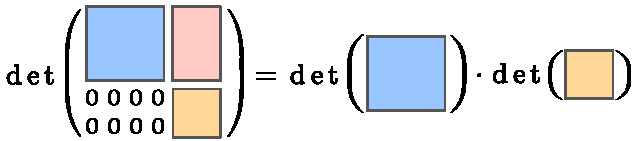
\includegraphics[width = 0.8 \columnwidth]{3_Determinante/Blocksatz.pdf}
\end{center}

\textbf{LR-Zerlegung} \par
\vskip1pt
Nur sinnvoll, wenn LR-Zerlegung bereits vorliegt. \par
\vskip4pt
$det(A) = (-1)^{\# Zeilenvertauschungen} \cdot r_{11} \cdot r_{22} \dotsm r_{nn}$

}
\WhiteSpace